\documentclass{article}
\usepackage[catalan]{babel}
\usepackage[latin1]{inputenc}   % Permet usar tots els accents i car�ters llatins de forma directa.
\usepackage{enumerate}
\usepackage{amsfonts, amscd, amsmath, amssymb}
\usepackage[pdftex]{graphicx}
\usepackage{longtable}

\setlength{\textwidth}{16cm}
\setlength{\textheight}{24.5cm}
\setlength{\oddsidemargin}{-0.3cm}
\setlength{\evensidemargin}{0.25cm} \addtolength{\headheight}{\baselineskip}
\addtolength{\topmargin}{-3cm}

\newcommand\Z{\mathbb{Z}}
\newcommand\R{\mathbb{R}}
\newcommand\N{\mathbb{N}}
\newcommand\Q{\mathbb{Q}}
\newcommand\K{\Bbbk}
\newcommand\C{\mathbb{C}}
\newcommand\cT{{\cal T}}
\def\fl{\text{fl}}
\def\pt{\text{pt}}
\def\fm{\text{fm}}

\newcounter{exctr}
\newenvironment{exemple}
{ \stepcounter{exctr} 
\hspace{0.2cm} 
\textit{Exemple  \arabic{exctr}: }
\it
\begin{quotation}
}{\end{quotation}}


\begin{document}

\begin{center}
\textbf{\Large Processament Digital del Senyal \\ Enginyeria T�cnica en Telem�tica \\ Examen Setembre 2011}
\end{center}

\begin{description}

\item[Problema 1]. 

\begin{enumerate}[a)]

\item Un sistema LTI respon a l'entrada $x_1=\{\underline{2}, -1\}$ amb la sortida $y_1=\{\underline{-2}, 1, 4, -2\}$.
Trobau la sortida corresponent a l'entrada $x_2=\{\underline{3}, 1, -1\}$.
\ \hfill{\textbf{ 4 pt.}}

\item Donat l'esquema de la figura seg�ent:

\begin{center}
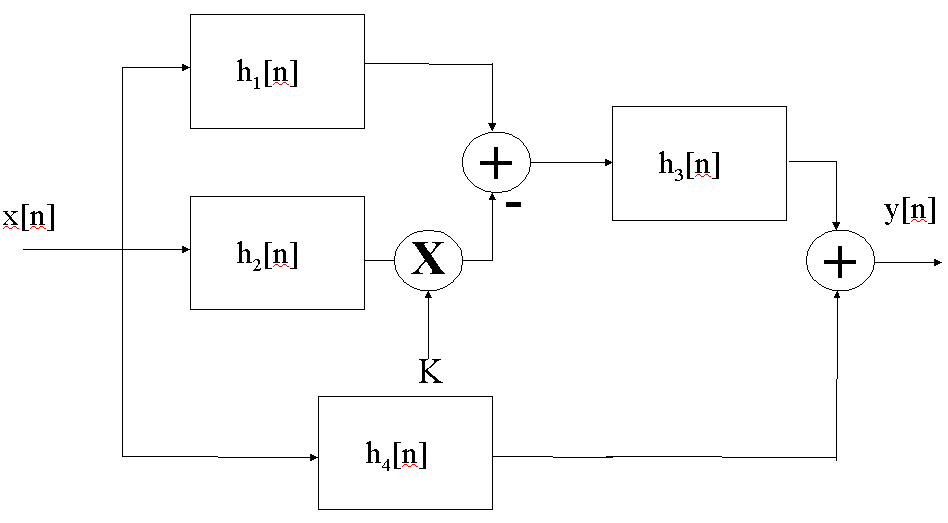
\includegraphics[width=10cm]{esquemaP1.png}
\end{center}

\noindent
on $h_1[n]=2 (\frac{1}{2})^n u[n]$, $h_2[n]=h_1[n-4]$, $h_3[n]=\{ \underline{-1}, 0, 1 \}$
i $h_4[n]=\{ \underline{a}, 0, b, 0, c, 0 \}$.

\vskip 0.3 cm
\noindent
Trobau els valors de les constants $K$, $a$, $b$ i $c$ que fan que el sistema es comporti com
un filtre FIR de fase lineal generalitzada de tipus IV.

\ \hfill{\textbf{ 6 pt.}}

\end{enumerate}

\vskip 0.5cm


\item[Problema 2].
Considerem un sistema LTI causal amb el diagrama de pols i zeros seg�ent, on tots els zeros i pols tenen multiplicitat 1:

\begin{center}
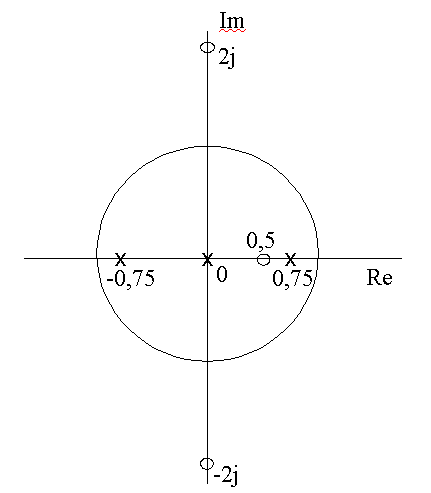
\includegraphics[width=4cm]{zerospols.png}
\end{center}

\begin{enumerate}[a)]

\item Trobau $H(z)$ sabent que $H(1)=2$.
\ \hfill{\textbf{ 2 pt.}}
\item Discutiu l'estabilitat del sistema.
\ \hfill{\textbf{ 1 pt.}}
\item Trobau la resposta impulsional del sistema.
\ \hfill{\textbf{ 5 pt.}}
\item Calculau la transformada Z de $(\frac{1}{4})^{2n}h[n-1]$
\ \hfill{\textbf{ 2 pt.}}


\end{enumerate}  

\newpage

\item[Problema 3].
Considerau el sistema digital de processament del senyal anal�gic de la figura seg�ent:


\begin{center}
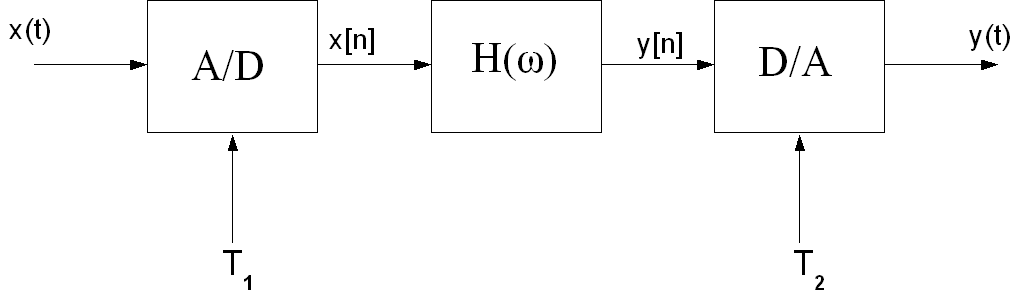
\includegraphics[width=10cm]{esquemaADDAT1T2.png}
\end{center}

\begin{center}
\begin{tabular}{cc}
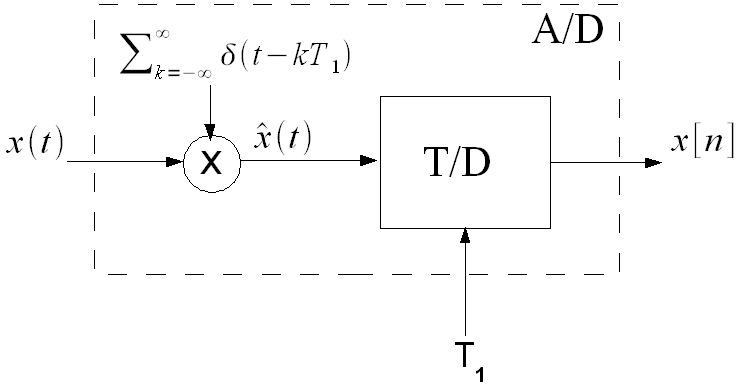
\includegraphics[width=6cm]{ADT1.png}
&
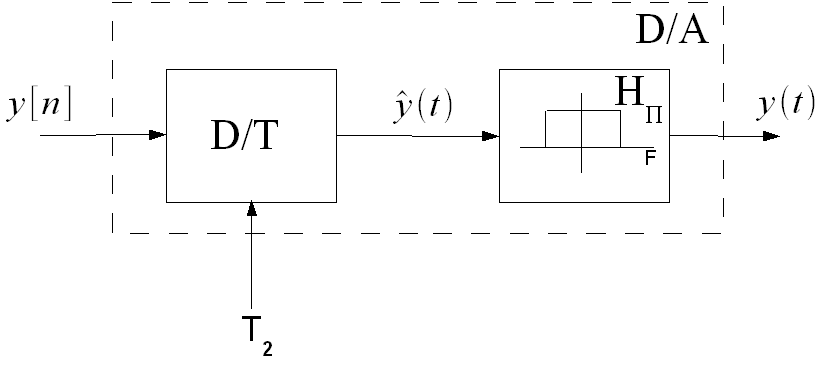
\includegraphics[width=6cm]{DAT2.png}
\end{tabular}
\end{center}

\noindent
Si sabem que els espectres dels senyals d'entrada i sortida s\'on, respectivament:

\begin{center}
\begin{tabular}{cc}
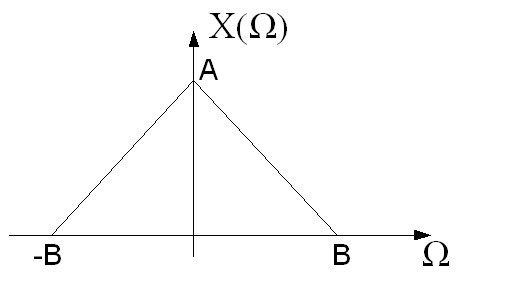
\includegraphics[width=6cm]{inputP3set.png}
&
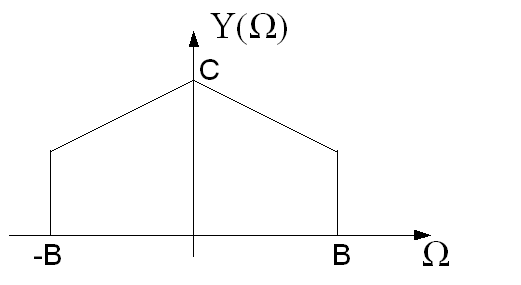
\includegraphics[width=6cm]{outputP3set.png}
\end{tabular}
\end{center}

\noindent
amb $B=2\pi \cdot 3000$.
Responeu raonadament a les seg�ents q�estions:


\begin{enumerate}[a)]
\item Calculau $T_1$ sabent que �s el m�xim periode de mostreig sense ali�sing.
 \ \hfill{\textbf{ 2 pt.}}

\item Sabent que $H(\omega)$ �s un filtre passa-baix ideal amb freq��ncia de tall $\omega_c$ i que $C=A/2$,
calculau $T_2$ i $\omega_c$ per obtenir a la sortida l'espectre que es mostra en la figura
anterior. Dibuixau l'espectre de tots els senyals
que intervenen en el sistema: $\hat{x}(t)$, $x[n]$, $y[n]$, $\hat{y}(t)$.
 \ \hfill{\textbf{ 8 pt.}}

\end{enumerate}

\vskip 0.5cm

\item[Problema 4].

\begin{enumerate}[a)]

\item Trobau l'expressi� m�s simplificada possible de la transformada de Fourier de
\[
h[n]=\{ -1, 2, 0, \underline{-1}, 0, 0, 0, 1, 0, -2, 1 \}
\]

\noindent
(Indicaci�: trobau la relaci� entre $h[n]$ i un senyal sim�tric $h'[n]$, calculau $H'(\omega)$ i
finalment trobau $H(\omega)$ a partir de $H'(\omega)$).

\ \hfill{\textbf{ 3 pt.}}

\item Trobau la resposta del sistema anterior a l'entrada
\[
x[n]=1-\frac{1}{3}\cos(\frac{\pi}{2}n+\frac{2\pi}{3})+2\sin(\frac{\pi}{4}n+\frac{\pi}{3})
\]

\ \hfill{\textbf{ 3 pt.}}


\item Un sistema causal t� per funci� de transfer�ncia:
  $$H(z)=\frac{(1-0.3z^{-1})(1+9z^{-2})}{(1-0.16z^{-2})}.$$

Trobau l'expressi� per a un sistema de fase m�nima $H_{\fm,1}$ i
    un sistema passa tot $H_\pt$ de manera que la composici� d'aquests
    ens doni el sistema original.
    
\ \hfill{\textbf{ 4 pt.}}


\end{enumerate}

\end{description}

\vskip 0.5cm

\noindent
Duraci� de l'examen: 4 hores.



\end{document}
